\documentclass[12pt,DIV14,BCOR10mm,a4paper,twoside,parskip=half-,headsepline,headinclude,english,ngerman,bibliography=totocnumbered]{scrreprt}

\usepackage{hshhelper_base}

%%%%%%%%%%%%%%%%%%%%%%%%%%%%%%%%%%%%%%%%%%%%%%%%%%%%%%%%%%%%%%%%%%%%%%%%%%
\begin{document}    % hier gehts los
  \thispagestyle{empty} % Titelseite

\includegraphics[width=0.2\textwidth]{Wortmarke_WI_schwarz}

   {  ~ \sffamily
  \vfill
  {\Huge\bfseries Bedrohungsanalyse}
  \bigskip

  {\Large
  Dennis Grabowski, Julius Zint, Philip Matesanz, Torben Voltmer \\[2ex]
  Masterprojekt \enquote{Entwicklung und Analyse einer sicheren Web-Anwendung} \\
  Wintersemester 18/19
 \\[5ex]
   \today }
}
 \vfill

  ~ \hfill
  
\includegraphics[height=0.3\paperheight]{H_WI_Pantone1665}

\vspace*{-3cm}

\tableofcontents  % Inhaltsverzeichnis

\printbibliography

\chapter{Zur Analyse verwendeten Methoden}
\section{Dataflow Diagram}

\begin{figure}[htbp]
  \hspace*{-1.75cm}
  \label{overview-dfd-pic}
  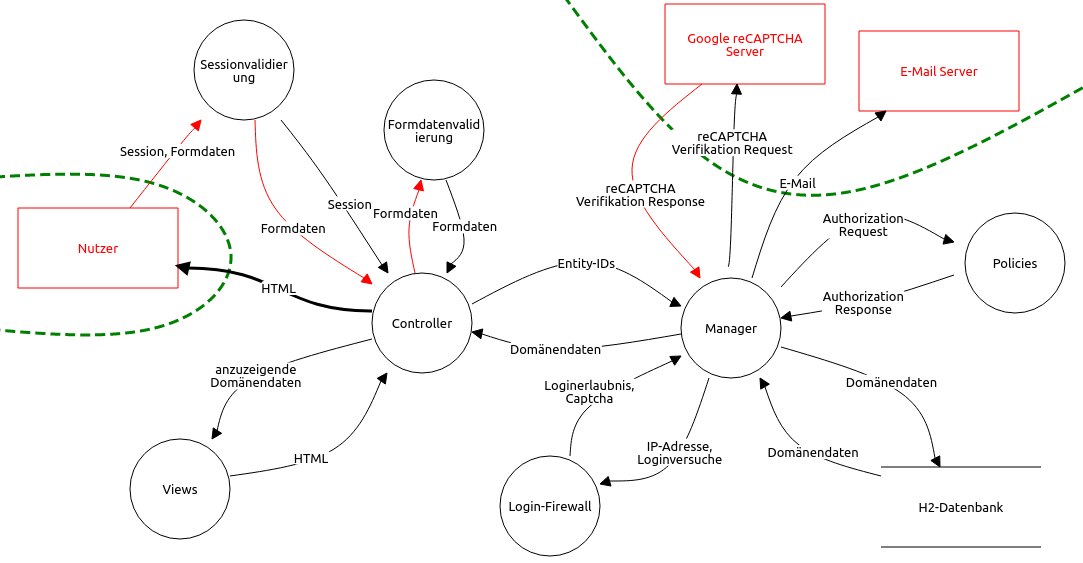
\includegraphics[width=1.25\linewidth]{resources/overview-dfd.jpg}
  \caption{Gesamtübersicht des Datenflusses in unserer Applikation}
\end{figure}

\subsection{Layered Entrypoints}

\renewcommand{\labelenumi}{\theenumi}
\renewcommand{\theenumi}{\arabic{enumi}}
\renewcommand{\labelenumii}{\theenumii}
\renewcommand{\theenumii}{\theenumi.\arabic{enumii}}
\renewcommand{\labelenumiii}{\theenumiii}
\renewcommand{\theenumiii}{\theenumii.\arabic{enumiii}}
\renewcommand{\labelenumiv}{\theenumiv}
\renewcommand{\theenumiv}{\theenumiii.\arabic{enumiv}}


\begin{enumerate}
  \item HTTP (Port 80)
  \begin{enumerate}
    \item \texttt{HomeController}
    \begin{enumerate}
      \item GET - \texttt{/}
    \end{enumerate}
    
    
 \item \texttt{LoginController}
    \begin{enumerate}
      \item \texttt{/login}
      \begin{enumerate}
        \item GET - \texttt{showLoginForm()}
        \item POST - \texttt{login(username, password, recaptcha)}
      \end{enumerate}
      \item \texttt{/logout}
      \begin{enumerate}
        \item POST - \texttt{logout()}
      \end{enumerate}
      \item \texttt{/changePasswordAfterReset}
      \begin{enumerate}
        \item GET - \texttt{showChangePasswordAfterResetForm}
        \item POST - \texttt{changePasswordAfterReset(username, currentPassword, password, passwordRepeat, recaptcha)}
      \end{enumerate}
    \end{enumerate}
    \item \texttt{UserController}
    \begin{enumerate}
      \item \texttt{/users}
      \begin{enumerate}
        \item GET - \texttt{showUsers()}
      \end{enumerate}
      \item \texttt{/users/create}
      \begin{enumerate}
        \item GET - \texttt{showCreateUserForm()}
        \item POST - \texttt{createUser(username, email)}
      \end{enumerate}
      \item \texttt{/users/delete}
      \begin{enumerate}
        \item POST - \texttt{deleteUser(userId)}
      \end{enumerate}
      \item \texttt{/resetpassword}
      \begin{enumerate}
        \item GET - \texttt{showResetUserPasswordForm}
        \item POST - \texttt{resetUserPassword(username)}
      \end{enumerate}
      \item \texttt{/sessions}
      \begin{enumerate}
        \item GET - \texttt{showActiveUserSessions()}
      \end{enumerate}
      \item \texttt{/sessions/delete}
      \begin{enumerate}
        \item POST - \texttt{deleteUserSession()}
      \end{enumerate}
    \end{enumerate}

   

    \item \texttt{GroupController}
    \begin{enumerate}
      \item \texttt{/user/groups}
      \begin{enumerate}
        \item GET - \texttt{showOwnGroups}
      \end{enumerate}
      \item \texttt{/groups}
      \begin{enumerate}
        \item GET - \texttt{showAllGroups}
      \end{enumerate}
      \item \texttt{/groups/create}
      \begin{enumerate}
        \item GET - \texttt{showCreateGroupForm}
        \item POST - \texttt{createGroup(groupname)}
      \end{enumerate}
      \item \texttt{/groups/:groupId}
      \begin{enumerate}
        \item GET - \texttt{showGroup(groupId)}
      \end{enumerate}
      \item \texttt{/groups/:groupId/members/remove}
      \begin{enumerate}
        \item POST - \texttt{removeGroupMember(groupId, userId)}
      \end{enumerate}
      \item \texttt{/groups/:groupId/members/add}
      \begin{enumerate}
        \item POST - \texttt{addGroupMember(groupId, userId)}
      \end{enumerate}
      \item \texttt{/groups/:groupId/delete}
      \begin{enumerate}
        \item POST - \texttt{deleteGroup(groupId)}
      \end{enumerate}
    \end{enumerate}
  \end{enumerate}
  \item SMTP (Port 587)
  \begin{enumerate}
    \item Versand der E-Mail für den Passwort-Reset (username, email, tempPassword)
  \end{enumerate}
\end{enumerate}


\section{STRIDE}
\chapter{Bedrohungen}
\section{Gefundene Bedrohungen}

\subsection{Globale Bedrohungen}

\begin{itemize}
  \item \textbf{Spoofing des Servers}
  \begin{itemize}
  \item Zweck: Damit der Nutzer einem die Daten darlegt
  \item Möglichkeiten:
  \item Risiko: Mittelmäßig
  \item Gegenmaßnahmen: Authentication des Servers via Certificate (HTTPS/TLS), HSTS
  \end{itemize}

  \item \textbf{Eavesdropping}
  \begin{itemize}
  \item Zweck:
  \item Möglichkeiten:
  \item Risiko: Mittelmäßig
  \item Gegenmaßnahmen: HTTPS + HSTS oder SecureCookie
  \end{itemize}

  \item \textbf{Replayattacken}
  \begin{itemize}
  \item Zweck:
  \item Möglichkeiten:
  \item Risiko: Mittelmäßig
  \item Gegenmaßnahmen: HTTPS / CSRF
  \end{itemize}

  \item \textbf{Tampering}
  \begin{itemize}
  \item Zweck:
  \item Möglichkeiten:
  \item Risiko: Mittelmäßig
  \item Gegenmaßnahmen: HTTPS/TLS
  \end{itemize}

  \item \textbf{Ungültig ausgestelltes Zertifikat (Türkischer Geheimdienst)}
  \begin{itemize}
  \item Zweck:
  \item Möglichkeiten:
  \item Risiko: Gering
  \item Gegenmaßnahmen: Cert Pinning
  \end{itemize}

  \item \textbf{DDOS (Out of scope)}
  \begin{itemize}
  \item Zweck: standard Zweck
  \item Möglichkeiten: standard means
  \item Risiko:
  \item Gegenmaßnahmen: None, or standard IDS
  \end{itemize}

  \item \textbf{XSS}
  \begin{itemize}
  \item Zweck:
  \item Möglichkeiten:
  \begin{itemize}
          \item Skript einbetten in Benutzername bei der Erstellung eines Nutzers
      \end{itemize}
  \item Risiko: Hoch
  \item Gegenmaßnahmen: CSP + alte Browser aussperren + Ausgabecodierung
  \end{itemize}
      Eingabevalidierung (Kleinbuchstaben und Zahlen, valide E-Mail-Adressen)

  \item \textbf{SQL Injection}
  \begin{itemize}
  \item Zweck:
  \item Möglichkeiten:
  \item Risiko: Hoch
  \item Gegenmaßnahmen:
  \begin{itemize}
    \item \texttt{ALLOW\_LITERALS=NONE}
    \item PreparedStatements
    \item Eingabevalidierung
  \end{itemize}
  \end{itemize}

  \item \textbf{CSRF}
  \begin{itemize}
  \item Zweck:
  \item Möglichkeiten:
  \begin{itemize}
          \item Einen fremden Benutzer ausloggen
          \item Einem Administrator einen Request unterjubeln, durch welchen er einen Nutzer erstellt
      \end{itemize}
  \item Risiko: Hoch
  \item Gegenmaßnahmen: CSRF-Tokens bei Requests checken
  \end{itemize}

  \item \textbf{Session fälschen (eine bestimmte oder irgendeine?)}
  \begin{itemize}
  \item Zweck: Client spoofen
  \item Möglichkeiten:
  \item Risiko: Hoch
  \item Gegenmaßnahmen: Signieren des Cookies durch PrivateKey und Verwendung von UUID, Bindung an IP-Adresse, Begrenzung der Lebenszeiten(?)
  \end{itemize}

  \item \textbf{Abstreitbarkeit illegaler Handlungen}
  \begin{itemize}
  \item Zweck:
  \item Möglichkeiten: Eintragen illegaler Namen bei Benutzernamen oder Gruppenmane
  \item Risiko: Gering
  \item Gegenmaßnahmen: Logging von IP + Zeit, Action, User
  \end{itemize}

  \item \textcolor{red}{Captcha lösen lassen von Indern?}
  \item \textcolor{red}{Elevation of privilege -> Frage an Peine. ?}
  \item \textcolor{red}{Security Header auflisten, warum welcher, wofür}
\end{itemize}

\subsection{Domänenspezifische Bedrohungen}

\subsubsection{Mögliche Angriffe auf den Loginprozess}

\begin{itemize}
  \item \textbf{Überlanges PW beim Login eingeben}
  \begin{itemize}
  \item Zweck: Zum DDOSn der Applikation
  \item Möglichkeiten: Durch Eingabe eines überlangen Passworts braucht der Hashing-Algorithmus sehr lange
  \item Risiko: Gering
  \item Gegenmaßnahmen: 
  \begin{itemize}
  \item Passwort-Länge mittels Eingabevalidierung beschränken
  \item Verwendung von bcrypt (lässt nur 72 Zeichen lange Passwörter zu, Lauzeit ist für alle Längen von Eingaben konstant)  
  \end{itemize}
\end{itemize}

  \item \textbf{Timing/Side-Channel auf Loginverhalten}
  \begin{itemize}
  \item Zweck: Herausfinden, ob Username existiert
  \item Möglichkeiten: Durch Messen der Antwortszeiten des Servers können Rückschlüsse darüber gezogen werden, welcher Code ausgeführt wurde (zB Hashing/DB-Zugriff)
  \item Risiko: Mittelmäßig-Hoch
  \item Gegenmaßnahmen: Loginprozess für jeden Fall gleich ablaufen lassen
  \end{itemize}

  \item \textbf{Online Brute-forcing}
  \begin{itemize}
  \item Zweck: Zum Knacken eines Benutzeraccounts
  \item Möglichkeiten: Beispielsweise durch Wörterbuchattacken
  \item Risiko: Hoch
  \item Gegenmaßnahmen:
  \begin{itemize}
      \item Captcha Mode = Login nur möglich, wenn Captcha gelöst wird.
      \item Accounts müssen nach x falschen Logins, einen Captcha lösen, sowie IP-Adressen sperren nach Y falschen Logins
      \item Schwache Passworter verbieten
      \item Zwei-Factor-Authentication
    \end{itemize}
  \end{itemize}
\end{itemize}

\subsubsection{Mögliche Angriffe beim Versand der Passwort-Reset-E-Mail}

\begin{itemize}
\item E-Mailversand abhören
  \begin{itemize}
  \item Zweck:
  \item Möglichkeiten:
  \item Risiko:
  \item Gegenmaßnahmen: SMTPS (Two-Faktor-Authentisierung)?
  \end{itemize}
\end{itemize}

\section{Ignorierte Bedrohungen}

\textcolor{red}{
Beispielsweise via Betriebssystem, physikalischer Zugriff auf der Maschine oder HTTPS?
Oder welche, für die es keine Motivation gibt, ggf. Repudiations
}

% Can be used to add a list of acronyms with their description
%\glsaddall
%\deftranslation{to=German}{Acronyms}{Abkürzungsverzeichnis}
%\deftranslation{to=German}{Glossary}{Glossar}
\printacronyms[title=Abkürzungsverzeichnis,toctitle=Abkürzungsverzeichnis]
\printglossary[type=main]

%\addcontentsline{toc}{chapter}{\listfigurename}
\listoffigures      % Abbildungsverzeichnis

%s\addcontentsline{toc}{chapter}{\listtablename}
% \listoftables       % Tabellenverzeichnis

\end{document}
